% !TEX program = lualatex
% !TEX options = -synctex=1 -interaction=nonstopmode "%DOC%"

\documentclass{report}

\title{Projet Python: L-System \\ Compte Rendu}
\author{\textsc{Brisset} Joachim \and \textsc{Kemgne} Jules-Antoine \and \textsc{Hopsore} Theo}
\date{\today}

\usepackage{luatextra}
\usepackage[a4paper, left=2cm, right=2cm, bottom=3cm, top=3cm]{geometry}
\usepackage[french]{babel}

\usepackage{fancyhdr}
\usepackage{lastpage}
\usepackage{hyperref}
\usepackage{smartdiagram} %create diagramm
%\usepackage{graphicx}
%\usepackage{array}
%\usepackage{hhline}
\usepackage{float} % use to force rendre of figure Here (H)

\renewcommand{\thesection}{\uppercase{\roman{section}}} % change theme of \section

\pagestyle{fancy}	
\fancyhf{}	

\fancyhead[l]{\textit{\rightmark}}
\fancyhead[C]{Projet Python : L-System} 
\fancyhead[r]{\textit{\today}}
\renewcommand{\headrulewidth}{0.2pt}

\fancyfoot[L]{}
\fancyfoot[C]{Page \thepage ~sur \pageref{LastPage}}
\fancyfoot[R]{
\includegraphics[scale=0.25]{images/CyTech_Logo.jpg}}

\begin{document}
	\maketitle
	\clearpage
	
	\tableofcontents{\thispagestyle{fancy}}
	\clearpage
	
	\section{Présentation}
		\paragraph{}
			Ce projet est l'évaluation finale du module python. Ce projet aura pour but de réalisé un programme capable de, a partir d'un fichier d'entrée normée représentant un L-System, générer un code permettant de le dessiner.
	\section{Caractéristique de Projet}
		\paragraph{Langage de programmation}
			Le programme finale devra être rédiger en langage Python étant donné que ce projet est l'évaluation finale de ce module.
		\paragraph{Entrée}
			le fichier d'entrée devra être sous la forme suivante: \\

			\fbox{\parbox{\linewidth\fboxrule\fboxsep}{
			\begin{tabular}{lll}
				axiome= &<chaine de caractère> \\
				regles= &<symbole> = <chaine de caractère> \\
						& \hspace{19mm} \vdots \\
						&<symbole> = <chaine de caractère> \\
				taille=	&<nombre> \\
				angle=	&<nombre> \\
				niveau=	&<nombre>
			\end{tabular}
			}}
	
			\subparagraph{} L'ordre de règles du fichier n'est pas considéré important. Cependant la présence et l'unicité des règles excepté "regles" est primordial. Il en vas de même si dans la règle "regles", un même symbole apparait plusieurs fois.
		
		\paragraph{Sortie} Le fichier de sortie doit être en langage Python pour pouvoir être exécuter immédiatement après.
	
	\section{Organisation}
		\paragraph{Git}
			Pour avoir un travail collaboratif efficace utilisons git, un logiciel qui permet de facilité le travail collaboratif sur les projets de programmation. Il permet a chacun de modifier le code sans trop se soucier des problèmes de modification simultanée, de garder une trace de toute nos modification du code et ainsi de revenir à un code antérieur si nécessaire, de travailler à part sur de nouvelle fonctionnalité en toute simplicité et revenir travailler sur le projet principal sans soucie.
			\subparagraph{}	
Le projet sera hébergé sur GitHub en version public.
			\subparagraph{}
Afin de facilité la vie a certain qui n'ont pas le courage d'apprendre le bash de git, nous utilisons gitKraken, une application permettant une utilisation intuitive de git a l'aide d'une interface graphique.
			\begin{figure}[h]
				\begin{center}			
					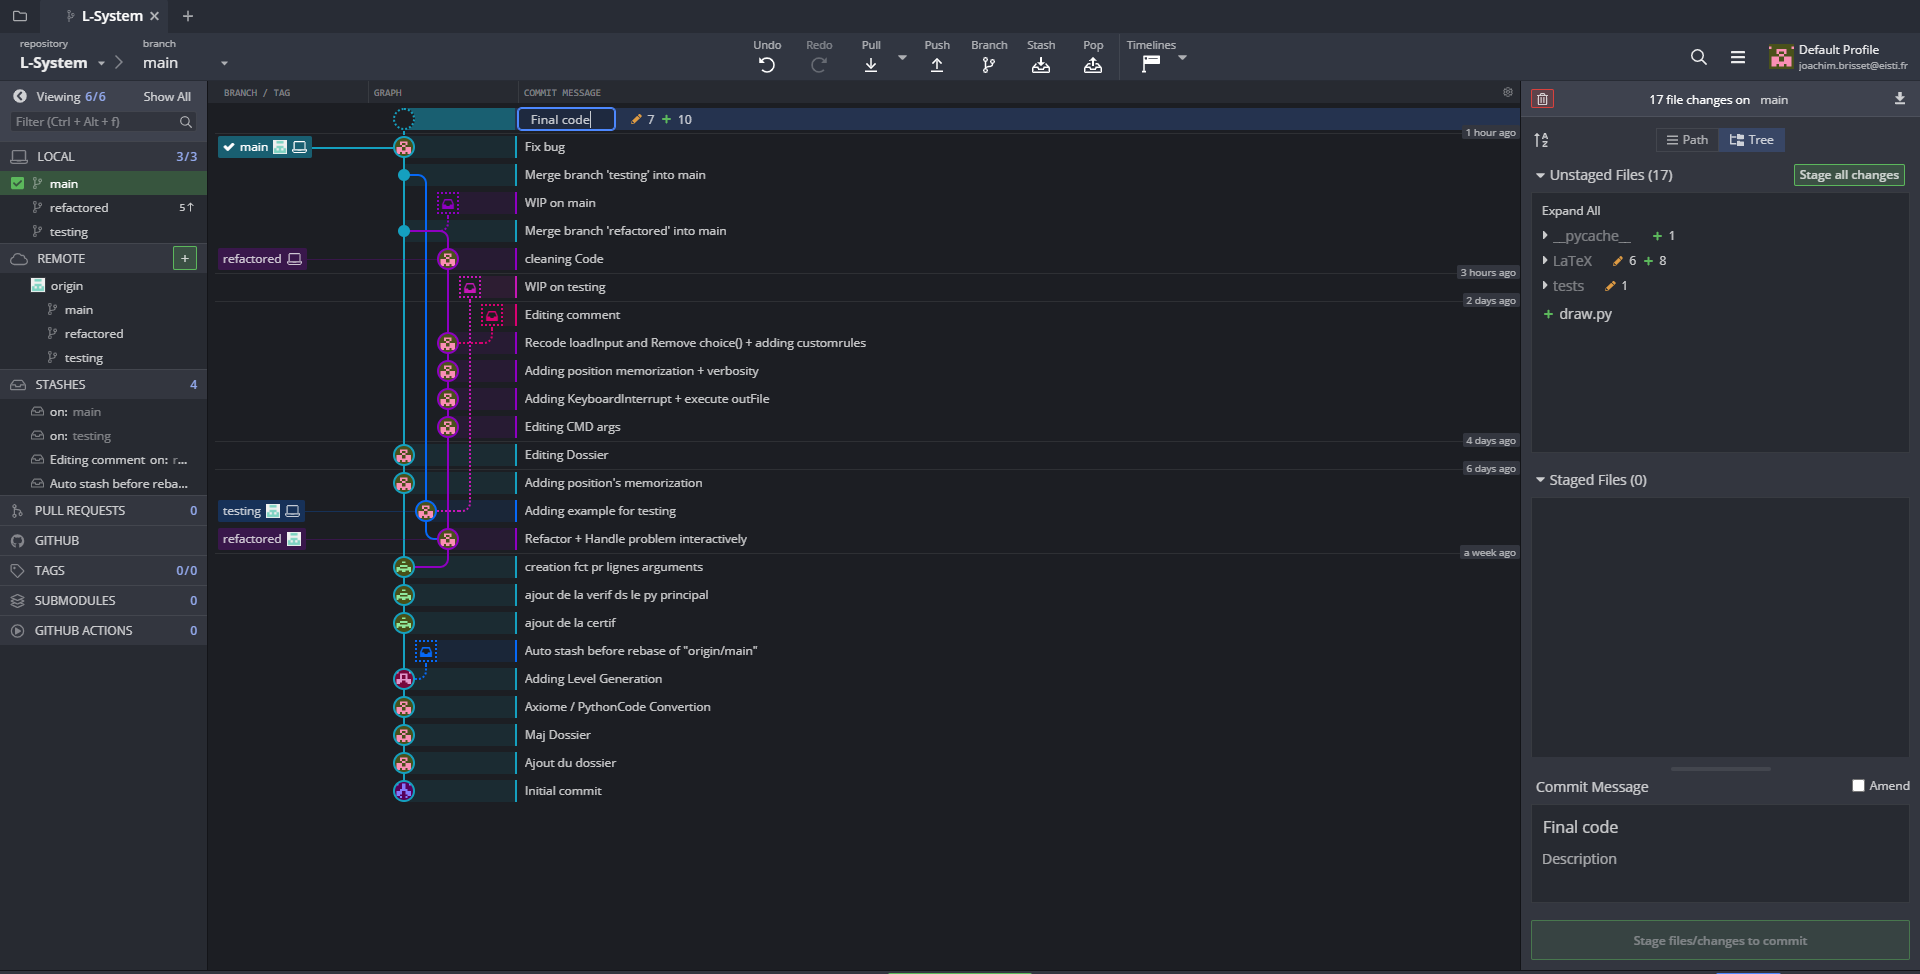
\includegraphics[scale=0.335]{images/gitkraken.PNG}
					\caption{screenshot de l'application GitKraken}
				\end{center}
			\end{figure}

		\paragraph{Processus de développement}
			Pour s'assurer que le programme fonctionnera convenablement nous nous sommes concentré tout d'abord sur le fonctionnement du programme sous sa forme la plus basique. C'est-à-dire que nous ne nous attardions pas sur les vérifications, interactivité du programme et tout autre ajout. A ce stade le programme ne peut que lire un fichier spécifique considéré valide et créer le code dans un autre fichier donné. Puis nous étendrons le programme en ajouter les vérification, l'interactivité et toutes autre fonctionnalités.
 
 		\paragraph{Planning de travail}
 			Pour être efficace dans le réalisation du projet nous avons commencé par réfléchir ensemble à la conception du programme pour ne pas trop revenir sur nos morceau de code précédent. Puis chaque semaine nous faisions un point sur l'avancement du projet aidions certain à finir le travail de la semaine précédente et enfin établissions le travail de chaque membre pour la semaine 
 	
 	\section{Conception}
 		\paragraph{Programme basique} Voici ci-dessous le processus du programme basique :
 		\begin{center}
			\smartdiagramset{
			uniform sequence color=true,
			sequence item text width=3cm,
			sequence item border color=white,
			sequence item font size=\footnotesize,
			sequence item text color=white
}
			\smartdiagram[sequence diagram]{
			Charger le L-System à partir du fichier,
			Croître le L-System au niveau voulu,
			Transcription en programme Python}
		\end{center}
		
		\subparagraph{}
			Chacune de ces étapes fera office d'un fonction a part entière
			
		\paragraph{Modèle du L-System}
			Le l-System est représenter par un dictionnaire avec les index suivant : axiome, regles, taille, angle, niveau. Généralement en programmation nous ecrivons en anglais, cependant pour facilité le programme et la compréhension nous préférerons utiliser les mots français qui seront les même que dans le fichier d’entrée. 
			
			\begin{figure}[h]
				\begin{center}			
					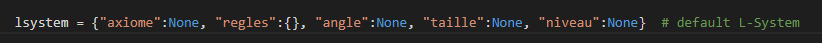
\includegraphics[scale=0.70]{images/modele_lsystem.PNG}
					\caption{modélisation en code Python du L-System}
				\end{center}
			\end{figure}
			
		\paragraph{Structure}
			Le projet n’étant pas très complexe nous avons décidé de rassembler l’intégralité programme dans un seul fichier, nommé \emph{l-system.py}, et de le décomposé en plusieurs fonction effectuant chacune une tâche particulière.
	\section{Développement}
		\subsection{Programme basique}
			\paragraph{} Dans sa version basique, le programme n'est pas très compliqué, on n'y distingue que trois fonctionnalités importantes:
				\subparagraph{•}
				En premier lieu, le chargement du L-System par la lecture d'un fichier: \\
				Fonction de tri (load input)
				Cette fonction va lire ligne par ligne de lsysteme afin de pouvoir créer des variables compréhensibles par le programme , elle va aussi verfier que toutes les instructions énoncées éxistes bien , qu'il n'y a pas plusieurs occurences pour une même règle.
				
				\subparagraph{•}
				Puis ensuite la croissance du L-System jusqu'au niveau souhaité:
				Cette tâche est assuré par la fonction \emph{generate\_L\_System\_by\_Level}. Le rôle de cette fonction est de générer le nouvel axiome à partir des règles de construction jusqu'au niveau de croissance voulu.
				Lap première boucle sert a repeter la tâche jusqu'aux niveau souhaité et la seconde boucle de parcourir tout l'axiome caractère par caractère et de remplacer les caractère remplacable. 

				\begin{figure}[h]
					\begin{center}
						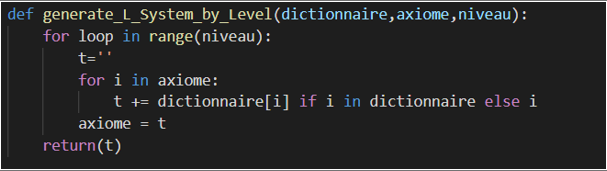
\includegraphics[scale=0.70]{images/generatebylevel.PNG}
						\caption{fonction generate\_L\_System\_by\_Level}
					\end{center}
				\end{figure}
				
				\subparagraph{•}
				Et enfin la transcription du L-System en un code python capable de le dessiner. Cette fonctionnalité se fait au travers de l'appel de la function \emph{LSystemToPythonCode()} qui prend en paramètre l'axiome a dessiner (on aurait pu prendre le L-System en entier) et le nom du fichier de sortie. \\
				
				Les instructions associées a leur symbole sont stocké dans un dictionnaire:
				
				\begin{figure}[h]
					\begin{center}
						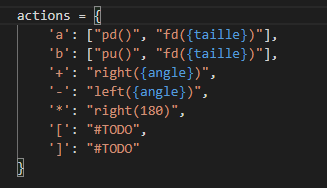
\includegraphics[scale=0.70]{images/action_switcher.PNG}
						\caption{pas de titre}
					\end{center}
				\end{figure}
			
				La notation \emph{\{taille\}} et \emph{\{angle\}} sont appelé placeholder, ce sont des variable qui seront remplacer par autre chose plus tard et notamment par leur valeur dans ce programme. \\
			
				Par la suite la fonction na plus qu'a écrire les ligne obligatoire tel que \emph{from turtle import *} et pour chaque symbol qu'elle rencontre dans l'axiome elle cherche les instruction associé et les écrit dans le fichier et finit son exécution

			\paragraph{Memorisation de la position} Une autre fonctionnalité certe bien moins importante mais pas des moidres, la memorisation de la position, est assuré par les ligne de codes suivantes inseré au debut du fichier de sortie: 

			\begin{figure}[h]
				\begin{center}
					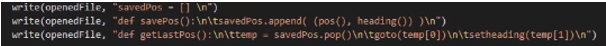
\includegraphics[scale=0.85]{images/position_memorisation.PNG}
					\caption{memorisation de la position}
				\end{center}
			\end{figure}
				
		\subsection{Vérification et Interactivité}
			\paragraph{}
			Fonction verification
			Cette fonction permet de verifier la validité des donnée entrées : elle vérifie que la type de variable associé à chaque instruction est correcte et vérifie aussi que leur validité (par exemple ne pas dépasser une valeur précise)

			\paragraph{} Ce programme permet à l’utilisateur de compiler avec  un nouveau fichier et a vérifier si le fichier est valide et excite.

			\begin{figure}[h]
				\begin{center}
					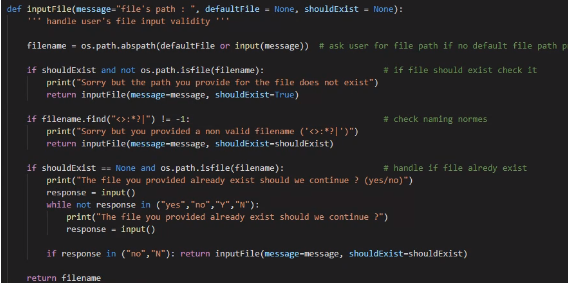
\includegraphics[scale=0.85]{images/interactions.PNG}
					\caption{interaction}
				\end{center}
			\end{figure}
			
		\subsection{Argument de commande}
			\paragraph{Fonction ligne de commande}
			Pour implementer cette fonctionnalité nous avons separer le code principale en 2 partie:
				\begin{itemize}
					\item la fonction \emph{app} qui est l'exécution de la fonctionnalité première du programme.
					\item la fonction \emph{main} qui vas gérer les argument et l'arret du programme et qui execute la fonction \emph{app}
				\end{itemize}
			La lecture des arguments est réalisé à l'aide du module emph{getopt} largement utilisé par la communauté et permet au programme d'interpreter des arguments de commande:
			\begin{itemize}
				\item le -i est associé au fichier d'entré 
				\item le -o à celui de sortie. 
				\item le --nodraw pour ne pas dessiner le L-System.
			\end{itemize} 
			Si il n'y a pas de fichier d'entré spécifié , ce dernier sera demandé au cours du programme , de meme , pour celui de sortie. 
			Si la syntax de la commande est est invalide l'utilisateur s'en voit informer par une aide.

			\begin{figure}[h]
				\begin{center}
					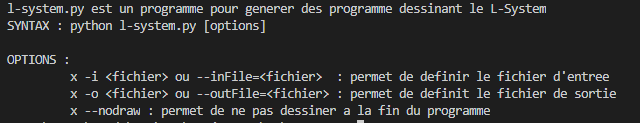
\includegraphics[scale=0.75]{images/exemple_help.PNG}
					\caption{exemple de l'aide du programme}
				\end{center}
			\end{figure}

		\subsection{Module}
			\paragraph{}
			Le fichier a été organisé de sorte à ce que'on puisse l'importer dans un autre projet si on le souhaite.

			\subparagraph{}
				Le code ne s'execute que si il est le fichier principal du projet.

				\begin{figure}[h]
					\begin{center}
						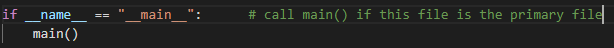
\includegraphics[scale=0.75]{images/modulePrimaryFile.PNG}
						\caption{Execution du programme en fichier principal}
					\end{center}
				\end{figure}

			\subparagraph{}
				De plus les fonctions ont été créer de sorte à ce que celle qui utilisé exclusivement par le programme pour sont bon fonctionnement soit privé et non accessible par l'import. Tandis que celle qui peuvent être utilile lors d'un import sont accessible et sont normalement independant des variables exterieurs ce qui les rend utilisable par d'autre developpeur et maniable par les paramètres.

				\begin{figure}[h]
					\begin{center}
						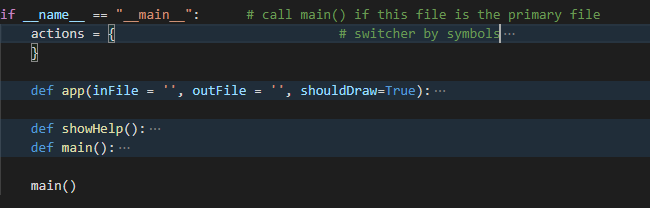
\includegraphics[scale=0.75]{images/privatefunctions.PNG}
						\caption{Exemples fonctions privées}
					\end{center}
				\end{figure}

				\begin{figure}[h]
					\begin{center}
						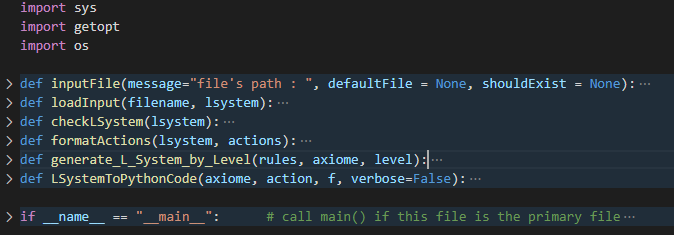
\includegraphics[scale=0.75]{images/fonctionpubliques.PNG}
						\caption{Fonctions publiques}
					\end{center}
				\end{figure}

		\subsection{En plus}
				\paragraph{Des actions customisables}
					Il est possible de rajouter et modifier des action associé au symbole dynamiquement a l'aide de la règles \emph{customrules}.

					\fbox{\parbox{\linewidth\fboxrule\fboxsep}{
						customrules=\\
						\hspace{19mm} "c=color("blue")" \\
						\hspace{19mm} "\#=width(5)"
					}}
				\subparagraph{}
					Il est même possible de mettre des scripts Python.

	\section{Acquis}
		\paragraph{with syntax} ???
		\paragraph{dict switcher}
			Durant le projet nous avons voulu utilisé un block switch pour pourvoir déterminer quelle instruction sont associé a un symbole néanmoins cette syntax n’existe pas en python ( bien qu’on aurait put utilise ‘if – elif’ ). Ce problème nous a amener a entrevoir une nouvelle utilisation des dictionnaire comme switcher grâce a « switcher[‘case’] ». De plus utilisé un dictionnaire de cette manière permet d’avoir un switch dynamique ( qui n’est pas fixe dans le programme) et ainsi de pouvoir le modifier pendant l’execution.
		\paragraph{type of input}
			On a appris a bien gérer le type d’entrée voulus a l’aide de la fonction input et du block try : except ValueError :
\end{document}